\chapter{Metodologia}

Este capítulo aborda o planejamento e execução do projeto, contendo os procedimentos e técnicas utilizadas, possibilitando a sua  replicação.

Tendo em vista os conceitos descritos nos capítulos anteriores, o presente trabalho tem como objetivo responder à seguinte questão problema:

\begin{center}
\textit{É possível extrair o perfil temático dos deputados através da análise dos seus discursos e proposições utilizando técnicas de aprendizado de máquina e processamento de linguagem natural?}
\end{center}

Além disso, será construído um \textit{website} com o intuito de fornecer uma forma melhor de visualização dos dados obtidos na análise dos discursos e proposições, através de gráficos interativos que garantam que o usuário tenha uma boa experiência ao utilizá-lo.


\section{Trabalhos Relacionados}

Durante a pesquisa bibliográfica realizada neste trabalho, encontrou-se alguns trabalhos que também fizeram análise de textos parlamentares utilizando aprendizado bayesiano. O Retórica Parlamentar\footnote{http://retorica.labhackercd.net/about.html}, idealizado por Davi Moreira\footnote{https://github.com/davi-moreira}, Manoel Galdino\footnote{https://github.com/mgaldino} e Luis Carli\footnote{https://github.com/luiscarli}, utiliza os discursos proferidos pelos parlamentares no Pequeno Expediente e no Grande Expediente da Câmara dos Deputados para promover a transparência do mandato e fornecer subsídios para o controle social com a divulgação dos temas mais debatidos em Plenário.

Entretanto, a técnica utilizada pelo Retórica para a classificação dos discursos é um modelo bayesiano hierárquico, descrito por \citeonline{grimmer2009}, onde através de aprendizado não supervisionado são gerados \(k\) \textit{clusters}, sendo \(k\) um valor escolhido ao executar o algoritmo. O resultado é exportado para o formato \textit{csv} e contém os termos mais frequentes de cada cluster. Um especialista deve ler e definir o rótulo de cada \textit{cluster}.

A visualização dos dados é feita através de um gráfico de bolhas, em que cada bolha representa a relevância (medido pela frequência) de cada tema dentre todos os deputados analisados. Dentro de cada bolha são colocados os deputados que enfatizam aquele tema nos seus discursos. Um deputado está associado a um único tema, que é o tema mais enfatizado por ele nos seus discursos.

\begin{figure}[h]
    \centering
    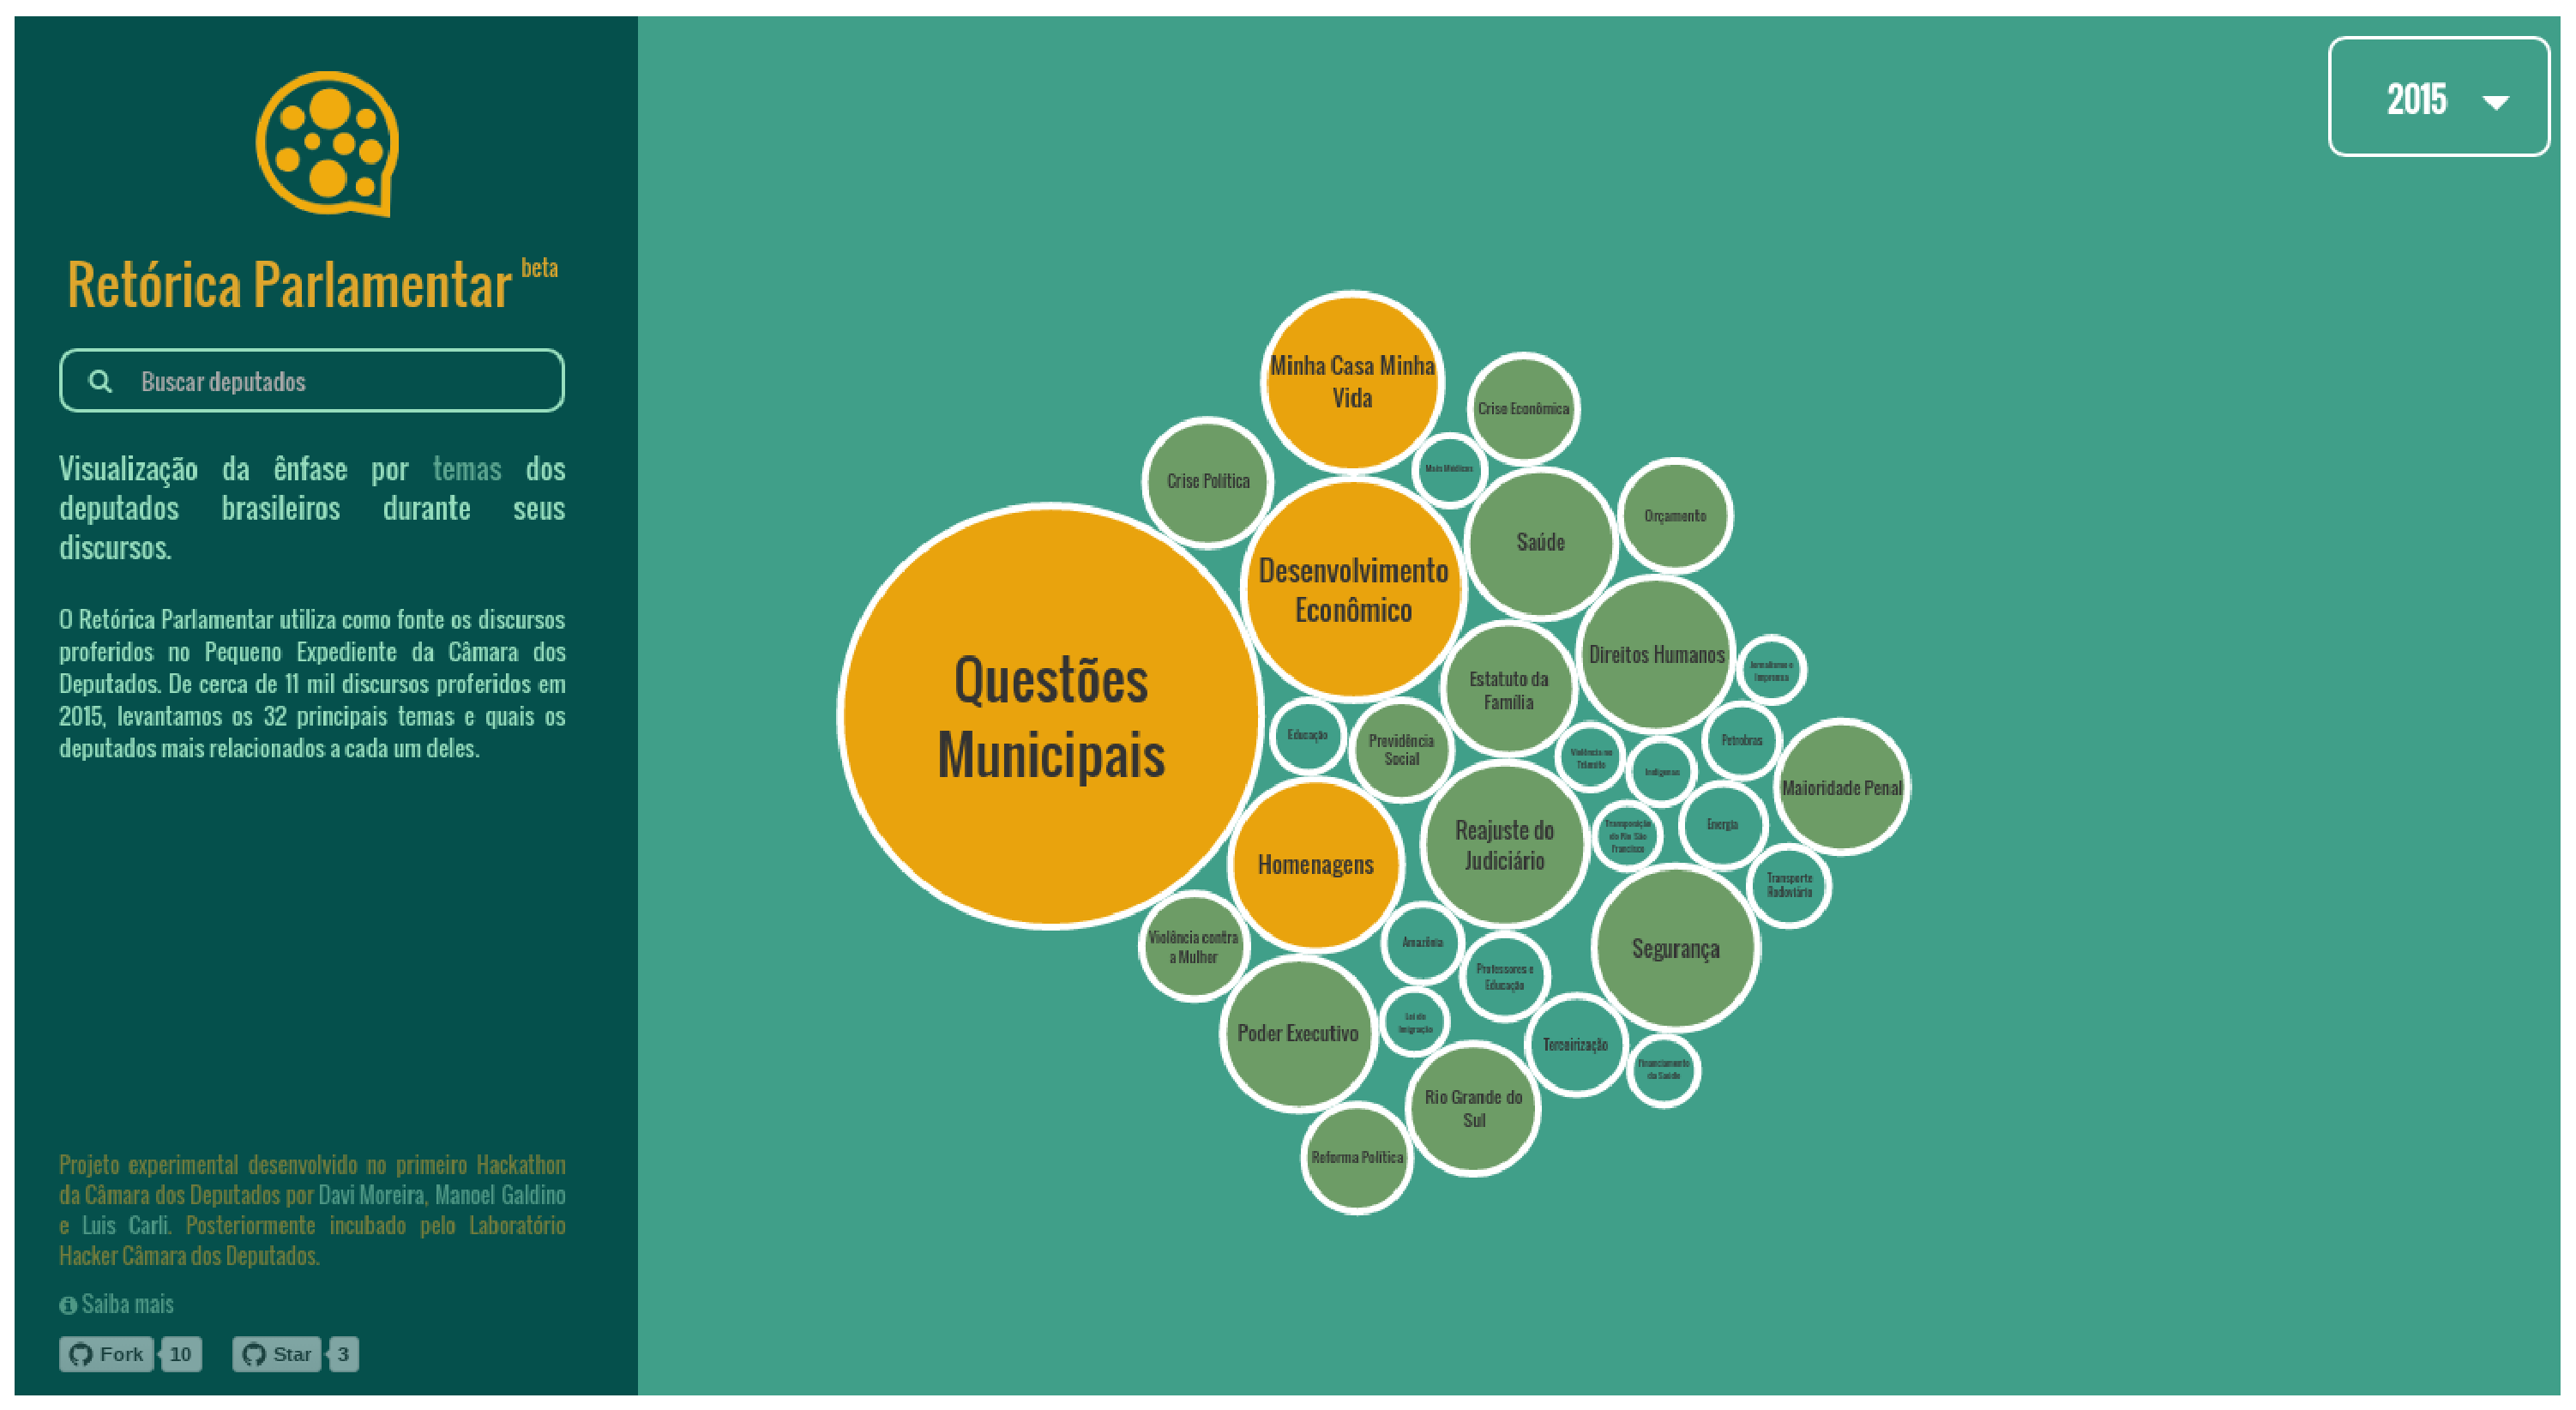
\includegraphics[scale=0.3]{figuras/retorica.eps}
    \caption{Retórica Parlamentar}
\end{figure}

